\documentclass{extbook}[14pt]
\usepackage{multicol, enumerate, enumitem, hyperref, color, soul, setspace, parskip, fancyhdr, amssymb, amsthm, amsmath, bbm, latexsym, units, mathtools}
\everymath{\displaystyle}
\usepackage[headsep=0.5cm,headheight=0cm, left=1 in,right= 1 in,top= 1 in,bottom= 1 in]{geometry}
\pagestyle{fancy}
\lhead{}
\chead{Answer Key for Module\,12M\,-\,Solving\,Word\,Problems Version C}
\rhead{}
\lfoot{Summer\,C\,2020}
\cfoot{}
\rfoot{}
\begin{document}
\textbf{This key should allow you to understand why you choose the option you did (beyond just getting a question right or wrong). \href{https://xronos.clas.ufl.edu/mac1105spring2020/courseDescriptionAndMisc/Exams/LearningFromResults}{More instructions on how to use this key can be found here}.}

\textbf{If you have a suggestion to make the keys better, \href{https://forms.gle/CZkbZmPbC9XALEE88}{please fill out the short survey here}.}

\textit{Note: This key is auto-generated and may contain issues and/or errors. The keys are reviewed after each exam to ensure grading is done accurately. If there are issues (like duplicate options), they are noted in the offline gradebook. The keys are a work-in-progress to give students as many resources to improve as possible.}

\rule{\textwidth}{0.4pt}

1. Determine the appropriate model for the graph of points below.
\begin{center} 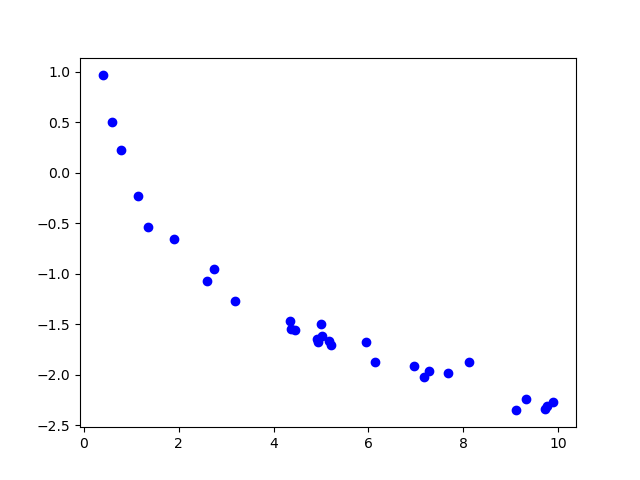
\includegraphics[width=0.3\textwidth]{../Figures/identifyModelGraph12C.png} \end{center} 

The solution is $ \text{Logarithmic model} $ 

\begin{enumerate}[label=\Alph*.] 
\item $ \text{Logarithmic model} $ 

 For this to be the correct option, we want a rapid change early, then an extremely slow change later. 
\item $ \text{Exponential model} $ 

 For this to be the correct option, we want an extremely slow change early, then a rapid change later. 
\item $ \text{Non-linear Power model} $ 

 For this to be the correct option, we need to see a polynomial or rational shape. 
\item $ \text{Linear model} $ 

 For this to be the correct option, we need to see a mostly straight line of points. 
\item $ \text{None of the above} $ 

 For this to be the correct option, we want to see no pattern in the points. 
\end{enumerate} 
 
\textbf{General Comment:} \textbf{General comments:} This question is testing if you can associate the models with their graphical representation. If you are having trouble, go back to the corresponding Core module to learn about the specific function you are having trouble recognizing. 

-----------------------------------------------

2. Solve the modeling problem below, if possible.
A new virus is spreading throughout the world. There were initially 3 many cases reported, but the number of confirmed cases has doubled every 3 days. How long will it be until there are at least 10000 confirmed cases? 
The solution is $ \text{About } 36 \text{ days} $ 

\begin{enumerate}[label=\Alph*.] 
\item $ \text{About } 36 \text{ days} $ 

 * This is the correct option. 
\item $ \text{About } 16 \text{ days} $ 

 You modeled the situation correctly but did not apply the properties of log correctly. 
\item $ \text{About } 25 \text{ days} $ 

 You modeled the situation with $e$ as the base, but solved correctly otherwise. 
\item $ \text{About } 14 \text{ days} $ 

 You modeled the situation with $e$ as the base and did not apply the properties of log correctly. 
\item $ \text{There is not enough information to solve the problem.} $ 

 If you chose this option, please contact the coordinator to discuss why you think this is the case. 
\end{enumerate} 
 
\textbf{General Comment:} \textbf{General Comments:} Set up the model the same as in Module 11M. Then, plug in 10000 and solve for $d$ in your model. 

-----------------------------------------------

3. For the scenario below, use the model for the volume of a cylinder as $V = \pi r^2 h$.
Pringles wants to add 35 \text{percent} more chips to their cylinder cans and minimize the design change of their cans. They've decided that the best way to minimize the design change is to increase the radius and height by the same percentage. What should this increase be? 
The solution is $ \text{About } 11 \text{ percent} $ 

\begin{enumerate}[label=\Alph*.] 
\item $ \text{About } 18 \text{ percent} $ 

 This corresponds to treating both radius and height as equal contributors and not solving correctly. 
\item $ \text{About } 3 \text{ percent} $ 

 This corresponds to not solving for the increase properly. 
\item $ \text{About } 16 \text{ percent} $ 

 This corresponds to solving correctly but treating both radius and height as equal contributors to the volume. 
\item $ \text{About } 11 \text{ percent} $ 

 * This is the correct option. 
\item $ \text{None of the above} $ 

 If you chose this, please contact the coordinator to discus how you solved the problem. 
\end{enumerate} 
 
\textbf{General Comment:} \textbf{General Comments:} Remember that when plugging the increases of values in, you need to treat it as that percentage above 100. For example, a 5 percent increase means 105 percent. 

-----------------------------------------------

4. Solve the modeling problem below, if possible.
In CHM2045L, Brittany created a 19 liter 31 percent solution of chemical $\chi$ using two different solution percentages of chemical $\chi$. When she went to write her lab report, she realized she forgot to write the amount of each solution she used! If she remembers she used 9 percent and 31 percent solutions, what was the amount she used of the 9 percent solution? 
The solution is $ -0.00 $ 

\begin{enumerate}[label=\Alph*.] 
\item $ 19.00 $ 

 This is the concentration of 31 percent solution. 
\item $ -0.00 $ 

 *This is the correct option. 
\item $ 9.50 $ 

 This would be correct if Brittany used equal parts of each solution. 
\item $ 10.36 $ 

 This was a random value. If this was not a guess, contact the coordinator to talk about how you got this value. 
\item $ \text{There is not enough information to solve the problem.} $ 

 You may have chose this if you thought you needed to know how much of the second solution was used in the problem. Remember that the total minus the first solution would give you the second amount used. 
\end{enumerate} 
 
\textbf{General Comment:} \textbf{General Comments:} Build the model exactly as you did in Module 9M. Then, solve for the volume you are looking for. 

-----------------------------------------------

0. Using the scenario below, model the population of bacteria $\alpha$ in terms of the number of minutes, $t$ that pass. Then, choose the correct approximate \textit{(rounded to the nearest minute)} replication rate of bacteria-$\alpha$.
A newly discovered bacteria, $\alpha$, is being examined in a lab. The lab started with a petri dish of 4 bacteria-$\alpha$. After 3 hours, the petri dish has 317 bacteria-$\alpha$. Based on similar bacteria, the lab believes bacteria-$\alpha$ doubles after some undetermined number of minutes. 
The solution is $ \text{About } 28 \text{ minutes} $ 

\begin{enumerate}[label=\Alph*.] 
\item $ \text{About } 171 \text{ minutes} $ 

 This solves for the constant correctly but converted incorrectly. 
\item $ \text{About } 389 \text{ minutes} $ 

 This does not solve for the constant correctly AND converted incorrectly. 
\item $ \text{About } 28 \text{ minutes} $ 

 * This is the correct option. 
\item $ \text{About } 64 \text{ minutes} $ 

 This does not solve for the constant correctly. 
\item $ \text{None of the above} $ 

 Please contact the coordinator to discuss why you believe none of the answers above are correct. 
\end{enumerate} 
 
\textbf{General Comment:} \textbf{General comments:} Your model should be $P(t) = P_0(b)^{kt}$, where $P(t)$ is the population at some time $t$, $P_0$ is the initial population, and $k$ is the replication rate. Be sure you convert the hours into minutes! 

-----------------------------------------------


\end{document}

